\subsection{Evaluation Paradigm Shift: From Output Scoring to Task-State Verification}
\headingnote{From ``Final-Answer Accuracy'' to ``Process Judgment'' and ``Task Closure''}


\begin{figure}[t]
    \centering
    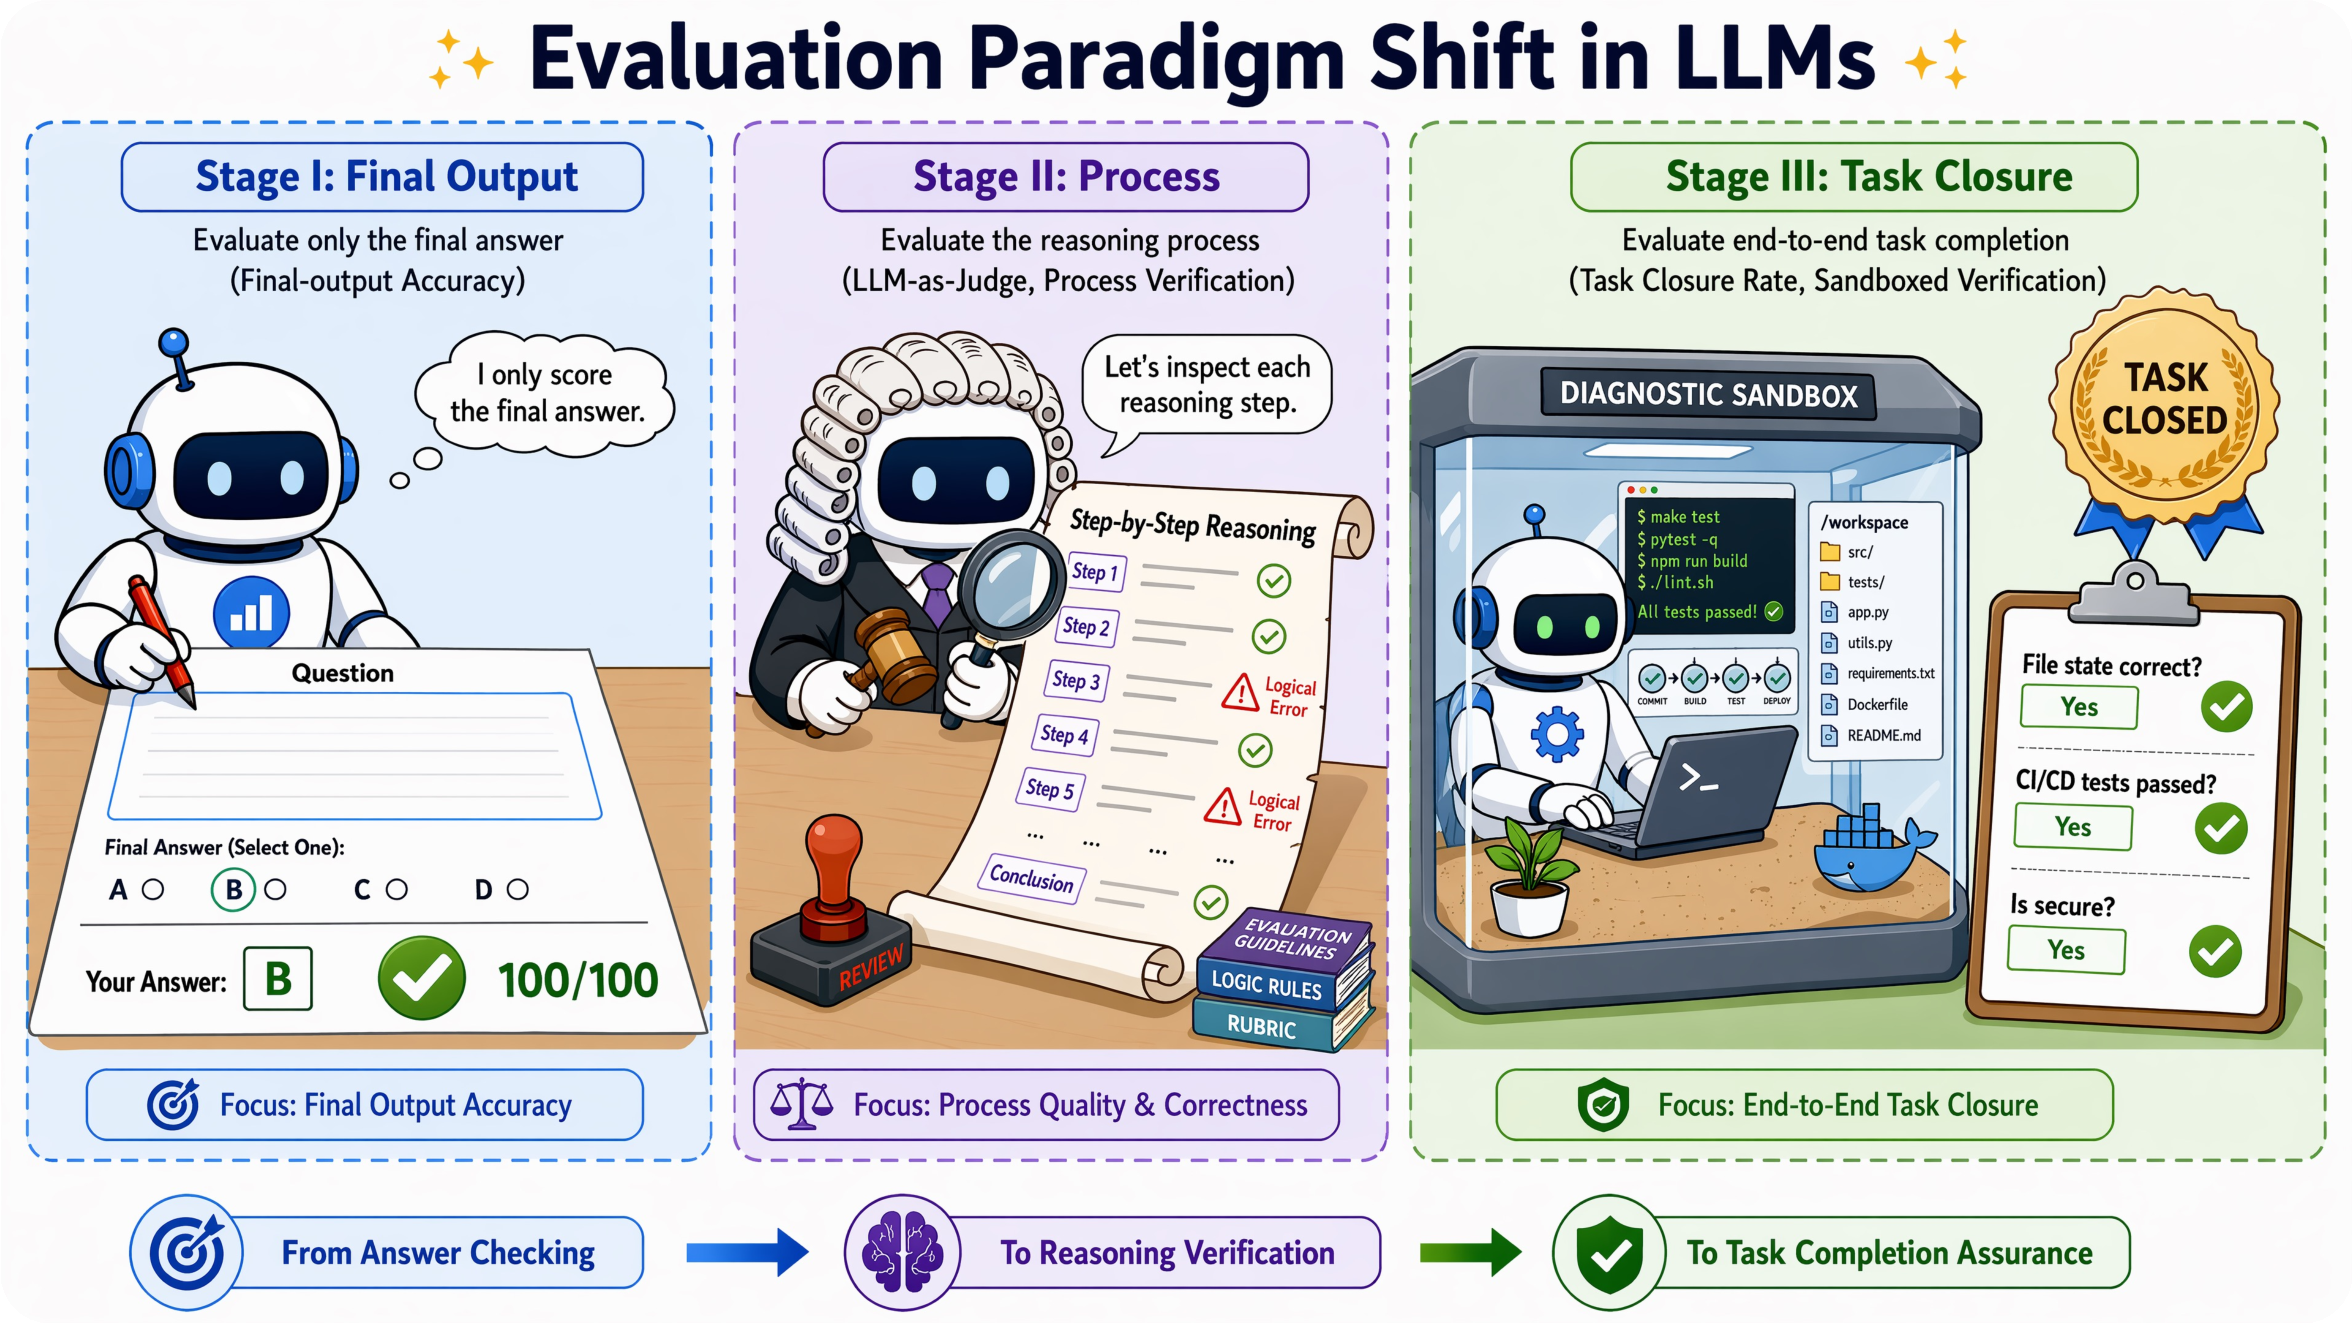
\includegraphics[width=\textwidth]{figure/eval.pdf}
    \caption{Evaluation paradigm shift: evaluation moves from final-answer correctness to process judgment and task closure. The figure summarizes how next-generation systems must be assessed by reasoning validity, environment state changes, reliability, efficiency, reproducibility, and safety.}
    \label{fig:eval}
\end{figure}

\begin{table}[!b]
\centering
\captionsetup{font=normalsize,skip=2pt}
\setlength{\tabcolsep}{1pt}
\renewcommand{\arraystretch}{2}
\caption{Summary of the evaluation paradigm shift from final-answer scoring to process judgment and workspace-level task closure.}
\label{tab:evaluation_paradigm_shift}
\fontsize{9pt}{8pt}\selectfont
\resizebox{\columnwidth}{!}{
\begin{tabular}{@{} p{0.1\columnwidth} p{0.20\columnwidth} p{0.23\columnwidth} p{0.2\columnwidth} p{0.25\columnwidth} @{}}
\toprule
\textbf{Stage} & \textbf{Evaluation Object} & \textbf{Core Metrics} & \textbf{Representative Benchmarks} & \textbf{Main Limitation} \\
\midrule

Final-Output Evaluation &
Static answers, labels, generated text, or executable final outputs &
Accuracy, exact match, BLEU/ROUGE, preference win rate, and Pass@1 &
MMLU, GSM8K / MATH, GPQA / FrontierMath, BIG-Bench / HELM &
Scores the endpoint but cannot reveal whether the model used a valid reasoning path or merely reached the right answer accidentally \\

Process-Level Evaluation &
Reasoning traces, intermediate steps, critiques, and verification paths &
Step correctness, judge preference, process-reward quality, consistency, and contamination resistance &
Hard2Verify / DeltaBench, ProcessBench / PRMBench &
Improves trace inspection but may rely on judge models, incomplete process labels, or reasoning that is not grounded in external state \\

Task-Closure Evaluation &
Interactive trajectories and final workspace states after tool, web, file, or UI operations &
Task success rate, final-state verification, tool-call efficiency, reliability, reproducibility, and trajectory-level safety &
SWE-bench, WebArena, OSWorld, ToolSandbox / $\tau$-bench &
Requires executable environments, reproducible initial states, trajectory logs, replay mechanisms, and costly final-state checks \\

Workspace OpenClaw Evaluation &
Persistent workspaces with skills, permissions, snapshots, external services, and auditable action chains &
Closure rate, unsafe-action rate, rollback behavior, skill stability, state diffs, auditability, and governance compliance &
Claw-Eval, ClawBench, ClawsBench, ATBench-Claw, ClawSafety &
Makes evaluation realistic but increases infrastructure cost, safety risk, simulator-design burden, and cross-run comparability challenges \\

\bottomrule
\end{tabular}
}
\end{table}


As shown in Figure~\ref{fig:eval}, evaluation evolves with the object being evaluated through three stages.
First, static-input tasks are scored by final-output correctness metrics such as accuracy~\citep{clawguard2026repo,caisi2026openclawcontrol,huntress2026fakeopenclaw,knownsec2026openclawsecurity,mitre2026openclawatlas}.
Second, long reasoning traces are inspected by LLM-as-a-judge and process-level verifiers for coherence, faithfulness, and correctness~\citep{oasis2026browserbackdoor,securityscorecard2026openclawexposure,gulyamov2026prompt,zhan2024injecagent}.
Third, agentic systems are judged by task closure: whether tool use and environment changes leave the workspace in a state that satisfies the user's intent.
Table~\ref{tab:evaluation_paradigm_shift} summarizes this shift from final-answer evaluation to process judgment and workspace-level task-state verification~\citep{derner2024security,mathew2024enhancing,debenedetti2024agentdojo,alnuaimi2025advancing,tanveer2026prompt}.


\subsubsection{Stage I: Final-Output Accuracy and Answer Correctness}

The first evaluation stage treats the model primarily as a generator of final answers. The central object is a single output: whether it matches a reference answer, satisfies a label, or is preferred as a response. For classification, multiple-choice QA, and short-answer reasoning tasks, simple metrics such as accuracy directly measure final-answer correctness. MMLU evaluates multi-subject knowledge through multiple-choice accuracy, while GSM8K and MATH evaluate mathematical reasoning by final-answer correctness \citep{hendrycks2020mmlu,cobbe2021gsm8k,hendrycks2021math}. Earlier generation metrics such as BLEU and ROUGE compare final text with references through n-gram overlap or summary similarity \citep{papineni2002bleu,lin2004rouge}. BIG-Bench and HELM broaden this paradigm across tasks and dimensions, but the evaluation unit remains the produced answer \citep{srivastava2022bigbench,liang2022helm,maloyan2026prompt,joseph2025prompt,kalliomaki2025large,li2026security,chhabra2025agentic}.

This initial stage is effective when the task has a clear label, executable answer, or reference output. It is also relatively easy to scale because outputs can be scored automatically. However, final-output accuracy has an important methodological limitation: it does not explain how the answer was obtained. A model may produce the correct answer for the wrong reason, or produce a wrong answer after an almost correct chain of reasoning. Therefore, as LLMs begin to solve harder problems through long reasoning traces, evaluation must move beyond Acc-style final-result scoring and ask whether the reasoning process itself is valid and reliable~\citep{gosmar2025prompt,vincent2025securing,yadav2025adversial,anand2026securing,li2025security}. Table~\ref{tab:stage1_final_output} lists representative models and methods under this traditional final-output evaluation setting.

\begin{table}[H]
\centering
\scriptsize
\setlength{\tabcolsep}{2pt}
\renewcommand{\arraystretch}{1.05}
\caption{Representative models and methods for Stage I final-output evaluation. Scores are reported under the original benchmark metrics; unavailable base models or unreported scores are denoted by ``-''. Rows sharing FastMCTS or CodeI/O citation numbers are variants or baselines reported in the same source paper.}
\label{tab:stage1_final_output}
\resizebox{\linewidth}{!}{
\begin{tabular}{@{} l|l|cccccc @{}}
\toprule
\textbf{Model} & \textbf{Base Model} & \textbf{MMLU} & \textbf{MMLU-Pro} & \textbf{GSM8K} & \textbf{MATH} & \textbf{MATH-500} & \textbf{HumanEval} \\
\midrule
GPT-5.4~\cite{openai2026gpt54} & - & 94.0 & 87.0 & 98.1 & 90.2 & - & 94.1 \\
Claude Opus 4.6~\cite{anthropic2026claudeopus46} & - & 92.1 & 82.5 & 97.8 & 91.5 & - & 92.4 \\
Gemini 3.1 Pro~\cite{google2026gemini31pro} & - & 92.6 & 91.2 & 94.2 & 85.3 & - & 87.6 \\
DeepSeek-V4-Pro-Base~\cite{deepseekai2026deepseekv4pro} & - & 90.1 & 73.5 & 92.6 & 64.5 & - & 76.8 \\
Qwen3.7 Max~\cite{qwen2026qwen37} & - & - & 89.6 & - & 94.6 & - & 92.4 \\
GLM-5.1~\cite{zai2026glm51} & - & 89.0 & 86.0 & 95.3 & 83.4 & - & 88.6 \\
SAGE-32B (Think)~\cite{jha2026sage} & Qwen2.5-32B~\cite{qwen2024qwen25} & 90.2 & 79.3 & 96.7 & - & 91.8 & - \\
Warmup K\&K~\cite{shrestha2025warmup} & Qwen2.5-14B~\cite{qwen2024qwen25} & - & 62.7 & - & - & 77.4 & - \\
AceMath-72B-Instruct~\cite{liu2024acemath} & Qwen2.5-Math-72B-Instruct~\cite{qwen2024qwen25math} & - & - & 96.4 & 86.1 & - & - \\
PromptCoT-DS-7B~\cite{zhao2025promptcot} & DeepSeek-R1-Distill-Qwen-7B~\cite{guo2025deepseek} & - & - & 92.6 & - & 93.0 & - \\
Nemotron-CrossThink-32B~\cite{akter2025nemotroncrossthink} & Qwen2.5-32B~\cite{qwen2024qwen25} & 83.6 & 69.4 & - & - & 84.0 & - \\
Introspective X Training~\cite{cui2026introspectivex} & - & 50.9 & 27.9 & 59.5 & 46.5 & - & 54.9 \\
CoT2-Meta~\cite{ma2026cot2meta} & Claude Sonnet 4.5~\cite{anthropic2025claudesonnet45} & - & 88.4 & 98.6 & 92.8 & - & 72.8 \\
Guideline Forest~\cite{chen2025guidelineforest} & GPT-4o-mini~\cite{openai2024gpt4omini} & - & - & 93.5 & - & 69.2 & 95.4 \\
STOP-ECN~\cite{xu2026stop} & DeepSeek-R1-Distill-Qwen-7B~\cite{guo2025deepseek} & - & - & 91.1 & - & 86.8 & - \\
FastMCTS+Branch-DPO~\cite{li2025fastmcts} & FastMCTS-7B & - & - & 89.9 & 75.4 & - & - \\
FastMCTS~\cite{li2025fastmcts} & Qwen2.5-7B~\cite{qwen2024qwen25} & - & - & 88.9 & 74.0 & - & - \\
Rejection Sampling~\cite{li2025fastmcts} & Qwen2.5-7B~\cite{qwen2024qwen25} & - & - & 87.1 & 70.0 & - & - \\
SBS~\cite{chen2024alphamath} & DeepSeek-Math-7B-Base~\cite{shao2024deepseekmath} & - & - & 84.1 & 66.3 & - & - \\
MCTS~\cite{chen2024alphamath} & DeepSeek-Math-7B-Base~\cite{shao2024deepseekmath} & - & - & 83.2 & 64.0 & - & - \\
DeepSeekMath-7B-RL~\cite{shao2024deepseekmath} & DeepSeekMath-7B~\cite{shao2024deepseekmath} & - & - & 88.2 & 51.7 & - & - \\
SimPO~\cite{novasky2025reduceoverthinking} & Qwen2.5-Math-7B-Instruct~\cite{qwen2024qwen25math} & - & - & 88.8 & 40.0 & 56.6 & - \\
Self-Explore~\cite{hwang2024self} & DeepSeek-Math-7B-Base~\cite{shao2024deepseekmath} & - & - & 78.6 & 37.7 & - & - \\
DeepSeek-Coder-V2-Instruct~\cite{deepseek2024coderv2} & - & - & - & 94.9 & 75.7 & - & 90.2 \\
OMI2 (Full)~\cite{li2025codei} & Qwen2.5-Coder-7B~\cite{qwen2024qwen25coder} & - & - & 88.5 & 73.2 & - & - \\
CODEI/O~\cite{li2025codei} & Qwen2.5-Coder-7B~\cite{qwen2024qwen25coder} & - & - & 86.4 & 71.9 & - & - \\
PyEdu~\cite{li2025codei} & Qwen2.5-Coder-7B~\cite{qwen2024qwen25coder} & - & - & 85.8 & 71.4 & - & - \\
MathCoder-CL~\cite{wang2024mathcoder} & Code-Llama-7B~\cite{roziere2023code} & - & - & 67.8 & 30.2 & - & - \\
\bottomrule
\end{tabular}
}
\end{table}


\begin{table}[H]
\centering
\tiny
\setlength{\tabcolsep}{1.0pt}
\renewcommand{\arraystretch}{1.03}
\caption{Representative models and methods for Stage II process-level reasoning evaluation. Scores are reported in the original benchmark metrics; unavailable base models or unreported scores are denoted by ``-''.}
\label{tab:stage2_process_level}
\resizebox{\linewidth}{!}{
\begin{tabular}{@{} l|l|cccccc|cccc|cccc|cccc @{}}
\toprule
\textbf{Model / Method} & \textbf{Base Model} &
\multicolumn{6}{c|}{\textbf{Hard2Verify}} &
\multicolumn{4}{c|}{\textbf{DeltaBench}} &
\multicolumn{4}{c|}{\textbf{ProcessBench}} &
\multicolumn{4}{c}{\textbf{PRMBench}} \\
\cmidrule(lr){3-8}\cmidrule(lr){9-12}\cmidrule(lr){13-16}\cmidrule(l){17-20}
 & &
\textbf{Step A} & \textbf{Step F1} & \textbf{Resp. A} & \textbf{Resp. F1} & \textbf{ErrID A} & \textbf{ErrID F1} &
\textbf{Avg.} & \textbf{HM} & \textbf{Corr.} & \textbf{Err.} &
\textbf{GSM8K} & \textbf{MATH} & \textbf{Olympiad} & \textbf{Omni} &
\textbf{Overall} & \textbf{Simp.} & \textbf{Sound.} & \textbf{Sens.} \\
\midrule
GPT-5~\cite{openai2025gpt5systemcard} & - & 86.5 & 85.8 & 89.7 & 89.5 & 70.6 & 69.7 & - & - & - & - & - & - & - & - & - & - & - & - \\
Gemini 2.5 Pro~\cite{google2025gemini25pro} & - & 83.4 & 83.1 & 85.7 & 85.5 & 52.5 & 52.5 & - & - & - & - & - & - & - & - & - & - & - & - \\
Claude Sonnet 4~\cite{anthropic2025claude4systemcard} & - & 70.6 & 60.4 & 78.2 & 73.4 & 53.5 & 39.3 & - & - & - & - & - & - & - & - & - & - & - & - \\
DeepSeek-R1~\cite{deepseek2025r1} & - & 68.9 & 62.3 & 74.0 & 72.8 & 54.2 & 45.4 & - & - & - & - & - & - & - & - & 67.8 & 62.9 & 71.4 & 77.1 \\
Qwen3-235B-A22B~\cite{qwen2025qwen3235bthinking2507} & - & 72.5 & 64.0 & 79.4 & 77.9 & 60.9 & 50.8 & - & - & - & - & - & - & - & - & - & - & - & - \\
Qwen3-Next-80B-A3B~\cite{qwen2025qwen3next80ba3binstruct} & - & 67.9 & 54.7 & 75.1 & 68.3 & 58.3 & 43.0 & - & - & - & - & - & - & - & - & - & - & - & - \\
GPT-4o~\cite{openai2024gpt4o} & - & - & - & - & - & - & - & 49.9 & 48.7 & 42.0 & 57.9 & 79.2 & 63.6 & 51.4 & 53.5 & 66.8 & 59.7 & 70.9 & 75.8 \\
o1-mini~\cite{openai2024o1systemcard} & - & - & - & - & - & - & - & - & - & - & - & 93.2 & 88.9 & 87.2 & 82.4 & 68.8 & 64.6 & 72.1 & 75.5 \\
Gemini-2.0-thinking-exp-1219~\cite{google2025gemini20flashthinking} & - & - & - & - & - & - & - & - & - & - & - & - & - & - & - & 68.8 & 66.2 & 71.8 & 75.3 \\
QwQ-32B-Preview~\cite{qwen2024qwqpreview} & - & - & - & - & - & - & - & - & - & - & - & 88.0 & 78.7 & 57.8 & 61.3 & 63.6 & 56.4 & 68.2 & 73.5 \\
Llama-3.3-70B-Instruct~\cite{meta2024llama33} & - & 54.3 & 18.4 & 57.0 & 28.2 & 49.4 & 2.5 & - & - & - & - & 82.9 & 59.4 & 46.7 & 43.0 & - & - & - & - \\
Qwen2.5-72B-Instruct~\cite{qwen2024qwen25} & - & 56.0 & 26.4 & 61.1 & 46.9 & 26.5 & 16.4 & - & - & - & - & 76.2 & 61.8 & 54.6 & 52.2 & - & - & - & - \\
Qwen2.5-14B-Instruct~\cite{qwen2024qwen25} & - & 60.5 & 47.6 & 63.4 & 63.2 & 43.5 & 18.9 & - & - & - & - & 69.3 & 53.3 & 45.0 & 41.3 & - & - & - & - \\
Qwen2.5-Math-72B-Instruct~\cite{qwen2024qwen25math} & - & - & - & - & - & - & - & - & - & - & - & 65.8 & 52.1 & 32.5 & 31.7 & 57.4 & 55.1 & 61.1 & 67.1 \\
\midrule
Qwen2.5-Math-PRM-72B~\cite{zhang2025qwenlessons} & Qwen2.5-Math-72B & 55.8 & 35.5 & 66.8 & 64.9 & 41.8 & 37.3 & - & - & - & - & 87.3 & 80.6 & 74.3 & 71.1 & 68.2 & 54.6 & 73.9 & 77.0 \\
Qwen2.5-Math-PRM-7B~\cite{zhang2025qwenlessons} & Qwen2.5-Math-7B & 57.6 & 42.4 & 63.1 & 57.6 & 35.0 & 32.5 & - & - & - & - & 82.4 & 77.6 & 67.5 & 66.3 & 65.5 & 52.1 & 71.0 & 75.5 \\
UniversalPRM-7B~\cite{tan2025aurora} & Qwen2.5-Math-7B-Instruct & 64.2 & 60.3 & 54.7 & 41.5 & 26.1 & 26.0 & - & - & - & - & 85.8 & 77.7 & 67.6 & 66.4 & - & - & - & - \\
ActPRM-X~\cite{duan2025activeprm} & Qwen2.5-Math-PRM-7B & - & - & - & - & - & - & - & - & - & - & 82.7 & 82.0 & 72.0 & 67.3 & 66.7 & 54.5 & 72.7 & 75.6 \\
ActPRM~\cite{duan2025activeprm} & Qwen2.5-Math-7B & - & - & - & - & - & - & - & - & - & - & 81.6 & 79.8 & 71.4 & 67.0 & 65.5 & 53.6 & 71.3 & 75.2 \\
RefCritic-R1-14B~\cite{tang2025refcritic} & DeepSeek-R1-Distill-Qwen-14B & - & - & - & - & - & - & - & - & - & - & 86.3 & 82.0 & 67.6 & 72.3 & - & - & - & - \\
RefCritic-Qwen-14B~\cite{tang2025refcritic} & Qwen2.5-14B-Instruct & - & - & - & - & - & - & - & - & - & - & 81.9 & 71.2 & 58.1 & 60.7 & - & - & - & - \\
FlexiVe (Think@64)~\cite{zhong2025sdv} & DeepSeek-R1-Distill-Qwen-14B & - & - & - & - & - & - & - & - & - & - & 88.1 & 90.1 & 86.7 & 80.4 & - & - & - & - \\
FlexiVe (Flex@128)~\cite{zhong2025sdv} & DeepSeek-R1-Distill-Qwen-14B & - & - & - & - & - & - & - & - & - & - & 83.0 & 85.0 & 80.0 & 75.2 & - & - & - & - \\
GenPRM-32B (Maj@8)~\cite{zhao2025genprm} & Qwen2.5-32B & - & - & - & - & - & - & - & - & - & - & 85.1 & 86.3 & 78.9 & 80.1 & - & - & - & - \\
GenPRM-7B (Maj@8)~\cite{zhao2025genprm} & Qwen2.5-7B & - & - & - & - & - & - & - & - & - & - & 81.0 & 85.7 & 78.4 & 76.8 & - & - & - & - \\
SPC (Round 2)~\cite{chen2025spc} & Qwen2.5-7B-Instruct & - & - & - & - & - & - & 60.5 & 59.5 & 68.2 & 52.8 & - & - & - & - & - & - & - & - \\
SPC (Round 1)~\cite{chen2025spc} & Qwen2.5-7B-Instruct & - & - & - & - & - & - & 58.8 & 57.3 & 68.4 & 49.3 & - & - & - & - & - & - & - & - \\
SPC (Round 0)~\cite{chen2025spc} & Qwen2.5-7B-Instruct & - & - & - & - & - & - & 54.9 & 53.5 & 45.9 & 64.0 & - & - & - & - & - & - & - & - \\
Qwen2.5-Math-7B-PRM800K~\cite{zheng2024processbench} & Qwen2.5-Math-7B & - & - & - & - & - & - & 58.5 & 41.3 & 90.1 & 26.8 & 68.2 & 62.6 & 50.7 & 44.3 & - & - & - & - \\
Pure-PRM-7B~\cite{cheng2025pure} & Qwen2.5-Math-7B & - & - & - & - & - & - & - & - & - & - & 69.0 & 66.5 & 48.4 & 45.9 & 65.3 & 52.2 & 70.2 & 75.8 \\
Skywork-PRM-7B~\cite{skywork2024prm} & Qwen2.5-Math-7B & 38.5 & 34.1 & 56.8 & 29.8 & 11.6 & 8.4 & - & - & - & - & 70.8 & 53.6 & 22.9 & 21.0 & 65.1 & 59.6 & 68.5 & 73.3 \\
Math-Shepherd-PRM-7B~\cite{wang2024math} & Mistral-7B & - & - & - & - & - & - & 53.3 & 14.3 & 7.7 & 98.8 & 47.9 & 29.5 & 24.8 & 23.8 & 47.0 & 47.1 & 45.7 & 60.7 \\
RLHFlow-PRM-Mistral-8B~\cite{xiong2024rlhflowmath} & Llama-3.1-8B & - & - & - & - & - & - & - & - & - & - & 50.4 & 33.4 & 13.8 & 15.8 & 54.4 & 46.7 & 57.5 & 68.5 \\
ReasonEval-34B~\cite{xia2024reasoneval} & CodeLlama-34B & - & - & - & - & - & - & - & - & - & - & - & - & - & - & 60.5 & 51.5 & 63.0 & 73.1 \\
ReasonFlux-PRM-7B~\cite{zou2025reasonfluxprm} & DeepSeek-R1-Distill-Qwen-7B & 53.1 & 22.4 & 55.9 & 53.8 & 42.5 & 28.7 & - & - & - & - & - & - & - & - & - & - & - & - \\
uPRM~\cite{gadetsky2026uprm} & Qwen2.5-Math-7B & - & - & - & - & - & - & - & - & - & - & 58.3 & 52.6 & 42.7 & 39.8 & - & - & - & - \\
\bottomrule
\end{tabular}
}
\vspace{2pt}
\noindent\parbox{\linewidth}{\normalsize \textit{Notes.} Hard2Verify reports Balanced Accuracy (A) and Balanced F1 for Step-Level, Response-Level, and ErrorID tasks. DeltaBench reports Average, harmonic mean (HM), correct-step recall, and error-step recall; the listed DeltaBench scores follow the comparison protocol in Chen et al.~\cite{chen2025spc}. ProcessBench columns report F1 on GSM8K/MATH/OlympiadBench/OmniMATH. PRMBench reports the overall PRMScore and category-average PRMScores for Simplicity, Soundness, and Sensitivity. Scores are taken from the corresponding benchmark papers or official benchmark result tables, while rows cite the model or method itself unless the method is a benchmark-trained baseline.}
\end{table}


\subsubsection{Stage II: LLM-as-Judge for Long-Chain Reasoning and Process Verification}

The second stage emerges when the model's output is no longer just an answer but a long reasoning chain. For Thinking LLMs, the evaluation target expands from is the final answer correct?'' tois the reasoning trajectory correct, coherent, and verifiable?'' Mathematical and scientific benchmarks such as AIME, GPQA, FrontierMath, Humanity's Last Exam, MMLU-Pro, and MMMU increase problem difficulty and make shallow answer matching less reliable \citep{rein2023gpqa,glazer2024frontiermath,phan2025hle,wang2024mmlupro,yue2023mmmu}. Code benchmarks provide process-sensitive verification: generated programs can be executed, and metrics such as Pass@1 test whether the first solution passes unit tests \citep{chen2021evaluating,jain2024livecodebench,evtimov2026wasp,geng2026prompt,chintala2025trustworthy,faccia2025prompting,wang2025comprehensive}.

In this stage, LLM-as-a-judge becomes essential as intermediate chains lack simple reference labels. Extending the pairwise preferences of MT-Bench and Chatbot Arena \citep{zheng2023judging}, judge models can inspect reasoning traces for step-by-step logic, hidden assumptions, and final support. ProcessBench and PRMBench make this process-level evaluation explicit by testing if models can identify incorrect intermediate steps \citep{zheng2024processbench,song2025prmbench}. Meanwhile, LiveBench and ARC-AGI-2 emphasize dynamic, abstraction-oriented evaluations to reduce contamination \citep{white2024livebench,chollet2025arcagi2}. Thus, evaluation shifts from scoring only endpoints to judging the long-chain reasoning process itself~\citep{wilson2024developer,del2025architecting,wang2026safeclaw,shah2026building,wang2026reframing,dong2024clr}. Table~\ref{tab:stage2_process_level} summarizes these representative methods and scores.


\begin{table}[H]
\centering
\scriptsize
\setlength{\tabcolsep}{2.4pt}
\renewcommand{\arraystretch}{1.05}
\caption{Representative models and methods for Stage III task-closure evaluation. Scores are original task success or pass rates; unavailable base models or unreported scores are denoted by ``-''.}
\label{tab:stage3_task_closure}
\resizebox{\linewidth}{!}{
\begin{tabular}{@{} l|l|cccccc @{}}
\toprule
\textbf{Model / Method} & \textbf{Base Model} & \textbf{SWE-V} & \textbf{Terminal 2.0} & \textbf{OSWorld-V} & \textbf{WebArena-V} & \textbf{BrowseComp} & \textbf{MCP-Atlas} \\
\midrule
GPT-5.4 xHigh~\cite{openai2026gpt54} & - & - & 75.1 & 75.0 & 67.3 & 82.7 & 67.2 \\
Claude Opus 4.6 Max~\cite{anthropic2026claudeopus46} & - & 80.8 & 65.4 & - & - & 83.7 & 73.8 \\
Gemini 3.1 Pro High~\cite{google2026gemini31pro} & - & 80.6 & 68.5 & - & - & 85.9 & 69.2 \\
DeepSeek-V4-Pro Max~\cite{deepseekai2026deepseekv4pro} & - & 80.6 & 67.9 & - & - & 83.4 & 73.6 \\
Kimi-K2.6 Thinking~\cite{moonshotai2026kimik26} & - & 80.2 & 66.7 & - & - & 83.2 & 66.6 \\
GLM-5.1 Thinking~\cite{zai2026glm51} & - & - & 63.5 & - & - & 79.3 & 71.8 \\
UI-TARS-2~\cite{bytedance2025uitars2} & UI-TARS-2 & 68.7 & 45.3* & - & - & 29.6* & - \\
OpenCUA-72B~\cite{wang2025opencua} & Qwen2.5-VL-72B & - & - & 45.0 & - & - & - \\
SWE-Exp~\cite{chen2025sweexp} & Claude 4 Sonnet & 73.0 & - & - & - & - & - \\
Kimi-Dev~\cite{kimiteam2025kimidevagentless} & Qwen2.5-72B-Base & 60.4 & - & - & - & - & - \\
SWE-Master-32B-RL~\cite{song2026swemaster} & Qwen2.5-Coder-32B & 61.4 & - & - & - & - & - \\
PDR+RTV~\cite{wang2026agentictts} & Gemini 3.1 Pro~\cite{google2026gemini31pro} & 76.6 & 64.8 & - & - & - & - \\
TACT-GATE~\cite{sui2026tact} & Qwen3.5-27B & 73.3 & 36.0 & - & - & - & - \\
IHR+NLAH~\cite{pan2026nlah} & GPT-5.4-mini & 73.0 & 53.9 & - & - & - & - \\
Polar RL (Pi)~\cite{xu2026polar} & Qwen3.5-4B & 40.4 & - & - & - & - & - \\
SA-SWE-32B~\cite{liu2025skyrlagent} & Qwen3-32B~\cite{qwen2025qwen3} & 39.4 & 16.3 & - & - & 19.4 (+) & - \\
CODESKILL~\cite{song2026codeskill} & Qwen3.5-35B-A3B & 66.0 & 34.1 & - & - & - & - \\
CodeScout-14B~\cite{sutawika2026codescout} & Qwen3-Coder-30B-A3B & 46.0 & - & - & - & - & - \\
TACO~\cite{ren2026taco} & MiniMax-M2.5~\cite{minimax2026minimaxm25} & - & 44.2 & - & - & - & - \\
ComputerRL~\cite{lai2025computerrl} & GLM-4.1V-9B-Thinking & - & - & 48.0 & - & - & - \\
UltraCUA-32B-RL~\cite{yang2025ultracua} & UltraCUA-32B & - & - & 43.7 & - & - & - \\
OS-Symphony~\cite{yang2026ossymphony} & GPT-5 & - & - & 65.8 & - & - & - \\
\bottomrule
\end{tabular}
}
\vspace{8pt}
\noindent\parbox{\linewidth}{\normalsize \textit{Notes.} SWE-V denotes SWE-bench Verified. OSWorld-V denotes OSWorld-Verified. WebArena-V denotes WebArena-Verified. Terminal 2.0 denotes Terminal-Bench v2.0. Retained columns were selected using Semantic Scholar citation-overlap among representative Stage III benchmark families and pruning redundant or less representative columns. Static frontier rows use one model source per row; Terminal 2.0, BrowseComp, and MCP-Atlas scores follow the DeepSeek-V4-Pro comparative report~\cite{deepseekai2026deepseekv4pro} unless an official row source reports the metric directly. Rows discovered through benchmark-overlap are included only when the source reports an end-to-end task-closure metric on a retained column. UI-TARS-2 scores marked with ``use the paper's extended GUI-SDK setting; its BrowseComp is BrowseComp-en. SA-SWE-32B reports BrowseComp-Plus, marked with(+)''.}
\end{table}

\subsubsection{Stage III: Agent \& OpenClaw Era: Task Closure Rate}

The third stage appears when LLMs become agents that operate tools, call APIs, browse websites, write files, and modify external environments. At this point, neither final-answer accuracy nor process judgment is sufficient. A reasoning trace may look valid, but the task is still incomplete if the code does not pass tests, the web order is not submitted, the document is not updated, or the calendar event is created with the wrong constraints. The evaluation target therefore becomes task closure: whether the system can transform an initial environment state into the intended final state. SWE-bench evaluates software-engineering agents by whether real GitHub issues are resolved through patches that pass tests, while WebShop and WebArena evaluate whether agents can complete interactive web tasks rather than merely describe how to do them \citep{jimenez2023swebench,yao2022webshop,zhou2023webarena}. Mind2Web, OSWorld, WorkArena, ToolSandbox, and $\tau$-bench broaden this closure-based perspective to offline web traces, desktop operating systems, enterprise workflows, stateful tool use, and multi-turn user-tool interaction \citep{deng2023mind2web,xie2024osworld,drouin2024workarena,lu2024toolsandbox,yao2024taubench,hutoward,grimes2025sok,pirch2026toward,dehghantanha2026sok,ray2025survey}. Table~\ref{tab:stage3_task_closure} compares representative task-closure evaluation results for agentic systems.



\begin{table}[H]
\centering
\tiny
\setlength{\tabcolsep}{1.0pt}
\renewcommand{\arraystretch}{1.05}
\caption{Representative models and methods for Stage IV workspace and OpenClaw evaluation. Scores are reported under the original benchmark metrics; lower ClawSafety ASR is better.}
\label{tab:stage4_workspace_openclaw}
\resizebox{\linewidth}{!}{
\begin{tabular}{@{} l|l|cc|c|ccc|ccc|c @{}}
\toprule
\textbf{Model / Method} & \textbf{Setting} & \multicolumn{2}{c|}{\textbf{Claw-Eval}} & \textbf{ClawBench} & \multicolumn{3}{c|}{\textbf{ClawsBench}} & \multicolumn{3}{c|}{\textbf{ATBench-Claw}} & \textbf{ClawSafety} \\
\cmidrule(lr){3-4}\cmidrule(lr){5-5}\cmidrule(lr){6-8}\cmidrule(lr){9-11}\cmidrule(l){12-12}
 & & \textbf{Gen.} & \textbf{Multi} & \textbf{SR} & \textbf{TSR} & \textbf{UAR} & \textbf{SCR} & \textbf{Acc.} & \textbf{F1} & \textbf{Rec.} & \textbf{ASR $\downarrow$} \\
\midrule
Claude Opus 4.6~\cite{anthropic2026claudeopus46} & OpenClaw on/on & 70.8 & 68.4 & - & 63.0 & 23.0 & 50.0 & - & - & - & - \\
Claude Sonnet 4.6~\cite{anthropic2026claudesonnet46} & OpenClaw / ClawSafety & 68.3 & 65.8 & 33.3 & 56.0 & 13.0 & 48.0 & - & - & - & 40.0 \\
MiMo-V2.5-Pro~\cite{xiaomi2026mimov25pro} & Claw-Eval & 64.0 & 63.2 & - & - & - & - & - & - & - & - \\
GLM-5.1~\cite{zai2026glm51} & Claw-Eval & 62.7 & 60.5 & - & - & - & - & - & - & - & - \\
Muse Spark~\cite{meta2026musespark} & Claw-Eval & 62.7 & 68.4 & - & - & - & - & - & - & - & - \\
Kimi K2.6~\cite{moonshotai2026kimik26} & Claw-Eval & 61.5 & 65.8 & - & - & - & - & - & - & - & - \\
GPT-5.4~\cite{openai2026gpt54} & OpenClaw on/on & 60.2 & 60.5 & 6.5 & 53.0 & 7.0 & 41.0 & - & - & - & - \\
DeepSeek V4 Pro~\cite{deepseekai2026deepseekv4pro} & Claw-Eval & 58.4 & 65.8 & - & - & - & - & - & - & - & - \\
Qwen3.6 Plus~\cite{qwen2026qwen36plus} & Claw-Eval & 57.1 & 65.8 & - & - & - & - & - & - & - & - \\
Qwen3.5-397B-A17B~\cite{qwen2026qwen35} & AgentDoG prompt & 57.8 & 52.6 & - & - & - & - & 83.8 & 86.5 & 87.5 & - \\
GLM-5~\cite{zeng2026glm5} & OpenClaw text-only / on/on & - & - & 24.2 & 60.0 & 23.0 & 48.0 & - & - & - & - \\
Gemini 3 Flash~\cite{google2025gemini3flash} & ClawBench & - & - & 19.0 & - & - & - & - & - & - & - \\
Claude Haiku 4.5~\cite{anthropic2025claudehaiku45} & ClawBench & - & - & 18.3 & - & - & - & - & - & - & - \\
Gemini 3.1 Flash-Lite~\cite{google2026gemini31flashlite} & OpenClaw on/on & - & - & 3.3 & 39.0 & 23.0 & 26.0 & - & - & - & - \\
Kimi K2.5~\cite{kimiteam2026kimik25} & OpenClaw / ClawSafety & 52.8 & 50.0 & 0.7 & - & - & - & - & - & - & 60.8 \\
Gemini 3.1 Pro~\cite{google2026gemini31pro} & OpenClaw on/on & 55.9 & 65.8 & - & 58.0 & 10.0 & 48.0 & - & - & - & - \\
Qwen3Guard-Gen-8B~\cite{qwen3guard2025} & Guard model & - & - & - & - & - & - & 52.1 & 36.3 & 23.1 & - \\
Llama-Guard-4-12B~\cite{meta2025llamaguard4_12b} & Guard model & - & - & - & - & - & - & 74.4 & 73.4 & 60.0 & - \\
ShieldAgent~\cite{chen2025shieldagent} & Guard model & - & - & - & - & - & - & 68.1 & 60.1 & 43.3 & - \\
Llama-3.3-70B-Instruct~\cite{meta2024llama33_70b_instruct} & AgentDoG prompt & - & - & - & - & - & - & 80.6 & 82.3 & 76.4 & - \\
AgentDoG-Qwen3-4B~\cite{liu2026agentdog} & AgentDoG & - & - & - & - & - & - & 87.2 & 89.6 & 92.9 & - \\
Gemini 2.5 Pro~\cite{google2025gemini25pro} & OpenClaw & - & - & - & - & - & - & - & - & - & 55.0 \\
DeepSeek V3~\cite{deepseek2024v3} & OpenClaw & - & - & - & - & - & - & - & - & - & 67.5 \\
GPT-5.1~\cite{openai2025gpt51} & OpenClaw & - & - & - & - & - & - & - & - & - & 75.0 \\
Claude Sonnet 4.6 + Nanobot~\cite{nanobot2026repo} & Nanobot scaffold & - & - & - & - & - & - & - & - & - & 48.6 \\
Claude Sonnet 4.6 + NemoClaw~\cite{nemoclaw2026} & NemoClaw scaffold & - & - & - & - & - & - & - & - & - & 45.8 \\
\bottomrule
\end{tabular}
}
\vspace{2pt}
\noindent\parbox{\linewidth}{\normalsize \textit{Notes.} Claw-Eval reports general and multi-turn PassAll$^3$ from the public leaderboard~\cite{ye2026claweval}. ClawBench reports live-web task success rate~\cite{zhang2026clawbench}. ClawsBench reports Task Success Rate (TSR), Unsafe Action Rate (UAR), and Safe Completion Rate (SCR) for OpenClaw on/on unless otherwise noted~\cite{li2026clawsbench}; on/on means domain skills on and meta prompt on. ATBench-Claw reports trajectory-safety Acc./F1/Recall, converted to percentages~\cite{yang2026atbenchclaw}. ClawSafety reports overall attack success rate (ASR), where lower is better~\cite{wei2026clawsafety}.}
\end{table}

\subsubsection{Stage IV: Workspace/OpenClaw Capability and Safety}

OpenClaw-oriented benchmarks make the task-closure view more explicit. ClawBench evaluates everyday online task completion, while ClawsBench evaluates productivity agents in simulated workspaces with services such as Gmail, Slack, Calendar, Docs, and Drive, combining capability and safety measurements under reproducible state management \citep{zhang2026clawbench,li2026clawsbench}. The metric stack, therefore changes again. Success rate measures whether the end-to-end task is completed. Reliability measures whether completion remains stable across long horizons, noisy observations, web layout changes, API failures, and partial mistakes. The efficiency measures tool calls, turns, tokens, wall-clock time, and human interventions. Reproducibility requires fixed initial states, state snapshots, trajectory logs, replayable actions, and final-state diffs. Without these controls, apparent success may be impossible to audit or compare~\citep{la2026design,hasan2026breaks,catalano2025agent,zhang2026litmus,ge2026governance}.

Safety and guardrails also become first-class evaluation targets in the task-closure stage. In a chatbot setting, an unsafe answer is usually a textual failure; in an agentic workspace, an unsafe action can leak private data, modify files, trigger external side effects, or execute an untrusted skill. ATBench-Claw evaluates trajectory-level safety diagnosis for OpenClaw-style agents, while ClawSafety, systematic OpenClaw security evaluation, and ClawKeeper highlight risks from prompt injection, unintended operations, malicious skills, privacy leakage, and weak runtime protection \citep{yang2026atbenchclaw,wei2026clawsafety,wang2026openclawsec,liu2026clawkeeper}. The evaluation paradigm, therefore, moves through three increasingly demanding objects: the final answer, the reasoning process, and finally the closed task state. Table~\ref{tab:stage4_workspace_openclaw} summarizes representative workspace/OpenClaw evaluation results across capability, reliability, and safety metrics.



\begin{AIbox}{Key Difference: Evaluation Object}
    \begin{itemize}[left=2pt,topsep=1pt,itemsep=2pt, parsep=1pt]
\item \textbf{Trend:} Evaluation is shifting from judging isolated final answers to inspecting reasoning trajectories and ultimately verifying whether the intended environment state has been achieved, \textit{thereby ensuring robust alignment with complex human objectives}.

\item \textbf{Challenge:} Task-closure evaluation requires reproducible initial states, trajectory logs, replayable actions, and final-state diffs; otherwise, agent success is difficult to audit or compare \textit{systematically across different models and complex environments}.
    \end{itemize}
\end{AIbox}


\section{Open Challenges and Future Directions}

\headingnote{From Model-Centric Capability to Ecosystem-Level Reliability}

The preceding sections have traced a clear trajectory from language generation to reasoning, tool use, and workspace-level task execution.
This progression marks a shift from AI systems that primarily answer questions to AI systems acting within digital environments.
However, greater autonomy also changes the nature of failure: errors are no longer limited to incorrect text, but may involve unsafe tool calls, corrupted workspace states, incomplete task closure, or untraceable long-horizon behavior.

This final section therefore focuses on the central challenge facing next-generation generative AI systems: how to make autonomy reliable in practice. We first summarize the open problems that prevent current agents from evolving into dependable digital colleagues. We then outline future directions toward self-evolving AI ecosystems, where models, contexts, tools, skills, workspaces, and governance mechanisms are engineered as an integrated whole.




\subsection{Open Challenges: Making Autonomy Reliable}
\headingnote{From Impressive Demonstrations to Dependable Digital Work}

As shown in Figure~\ref{fig:challenges}, despite significant recent progress, current LLM-based agents remain far from trustworthy digital workers. Their capabilities may appear impressive in isolated demonstrations, but real-world production deployment requires stable performance across long horizons, safe operation under strict permission constraints, persistent memory resisting collapse under growing context, and careful management of social and organizational consequences. The key challenge is not merely to make agents more capable, but to ensure that their autonomous behavior remains auditable, recoverable, controllable, and closely aligned with human values, ethical principles, and boundaries.

\subsubsection{Long-Horizon Reliability and Task Closure}
\headingnote{From Demonstrated Capability to Stable Completion}

The evaluation shift toward task closure reveals a major reliability bottleneck: an agent must not only reason correctly at individual steps, but also maintain progress until the intended environment state is achieved. Long-horizon tasks introduce several sources of instability. Errors can propagate across tool calls, partial failures can leave the workspace in inconsistent states, and early planning mistakes may only become visible after many irreversible actions.

Skill encapsulation partially mitigates this problem by turning common procedures into reusable units. However, composing skills into longer workflows introduces new interface-level failure modes. A skill may generate an output that is syntactically valid but semantically unsuitable for the next skill, while another may silently fail while leaving misleading traces. Therefore, reliable autonomy requires explicit mechanisms for progress monitoring, intermediate verification, self-healing, and recovery. Future systems need to detect when a trajectory is drifting away from the user's intent, repair local failures, and, when necessary, roll back to a safe checkpoint instead of continuing blindly.

\begin{figure}[t]
    \centering
    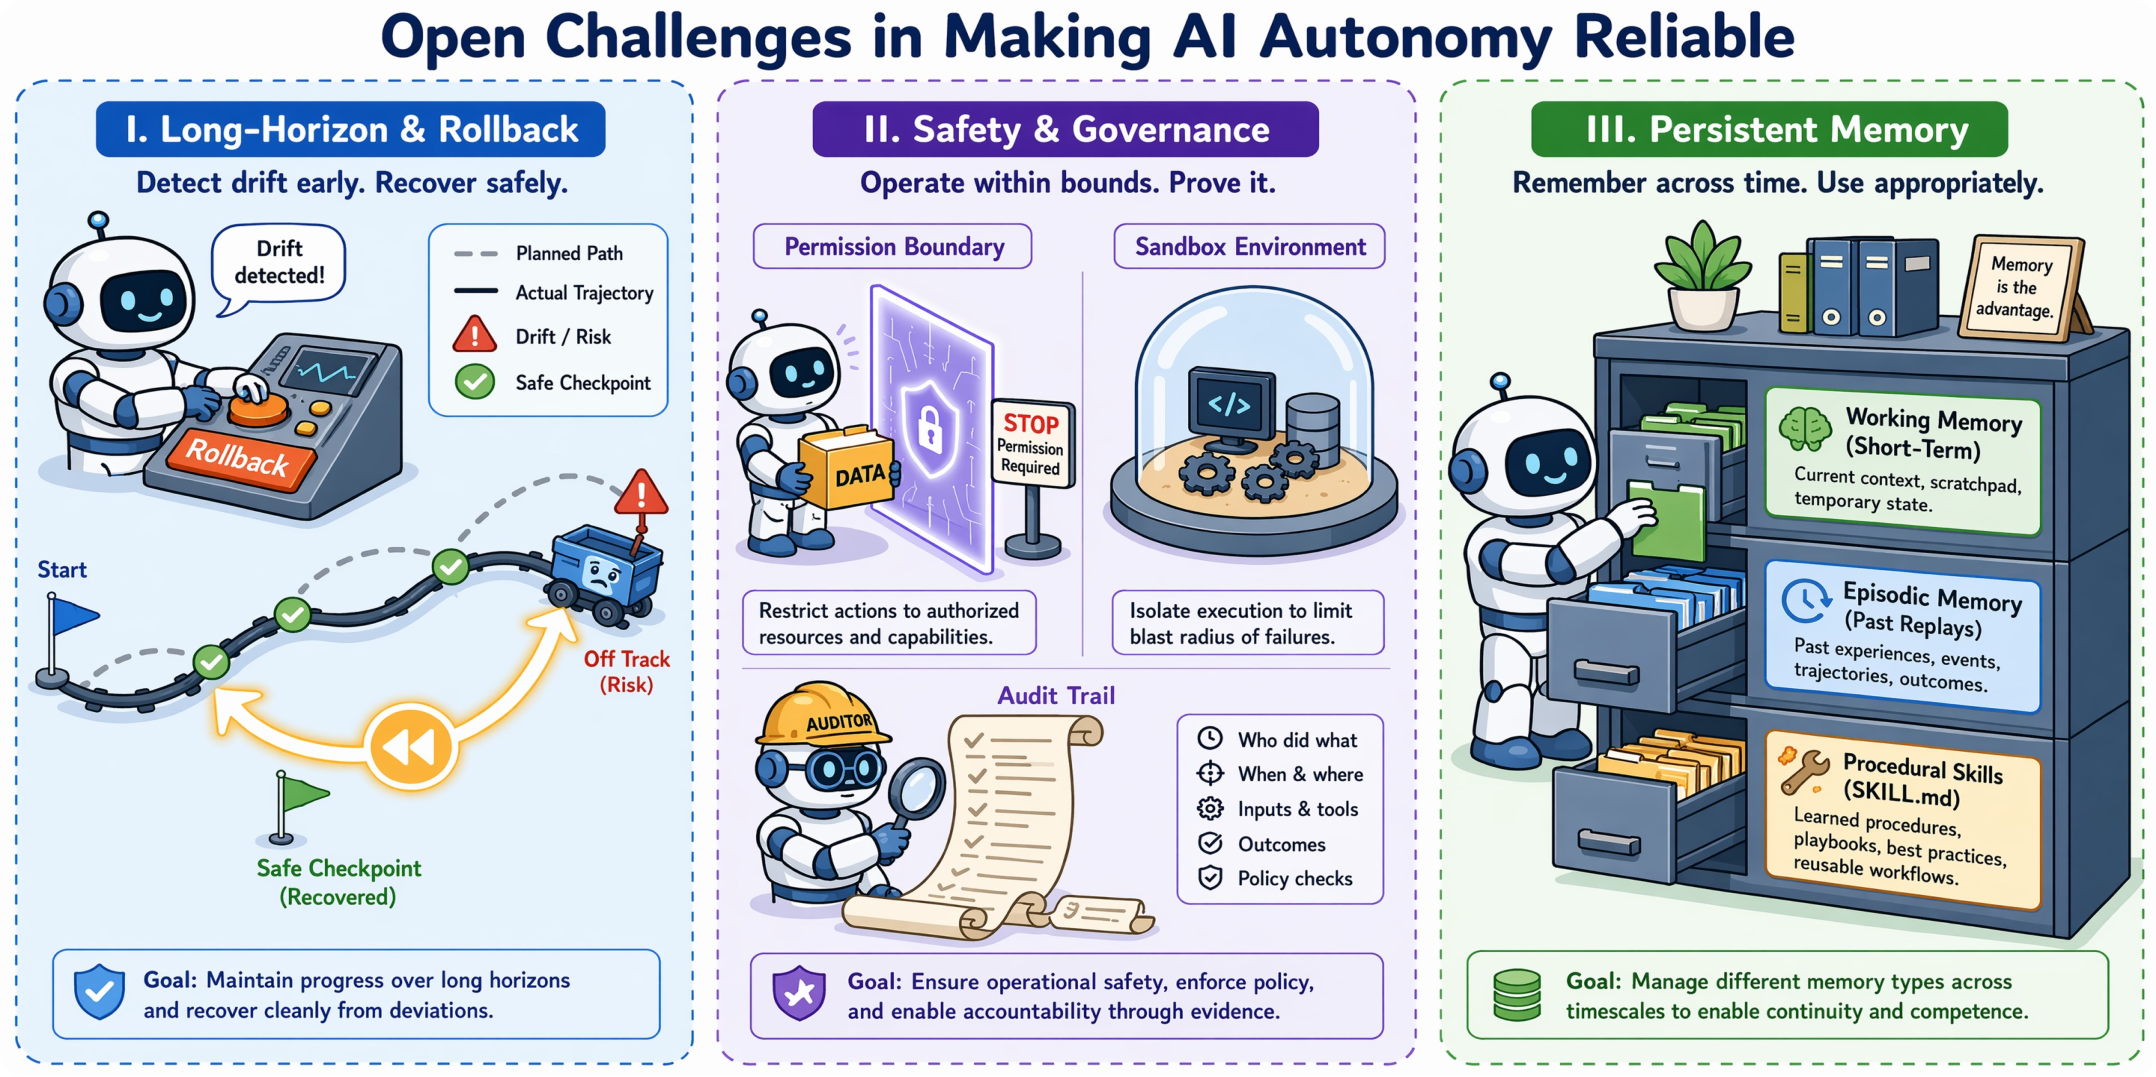
\includegraphics[width=\textwidth]{figure/challenges.pdf}
    \caption{Open challenges for reliable autonomy: as agents move from answering to acting in workspaces, failures become longer-horizon, stateful, and harder to reverse. The figure summarizes key bottlenecks around task closure, safety and governance, memory, context management, and persistent workspace state.}
    \label{fig:challenges}
\end{figure}

\subsubsection{Safety, Governance, and Permission Boundaries}
\headingnote{From Textual Guardrails to Operational Control}

As agents gain access to files, browsers, APIs, terminals, databases, and enterprise applications, safety must move beyond response filtering. In a chatbot setting, unsafe behavior often appears as harmful text; in an agentic workspace, unsafe behavior may leak private data, overwrite files, trigger external side effects, execute untrusted skills, or make unauthorized decisions. The safety problem therefore becomes operational rather than purely linguistic.

Reliable deployment of autonomous systems requires fine-grained permission isolation, risk-aware action validation, audit trails, and rollback mechanisms. Autonomous agents should operate within boundaries defining resource access, approval requirements, and logging or sandboxing. Human oversight must balance autonomy against operational risk. A central research challenge is building governance that preserves usefulness while keeping high-impact actions inspectable and controllable.

\subsubsection{Human--AI Collaboration Ethics and Data Boundaries}
\headingnote{From Technical Reliability to Socio-Technical Accountability}

Reliable autonomy is fundamentally a complex socio-technical problem. As agents become digital colleagues, they reshape who can participate in professional work and how that work is organized. On one hand, workspace agents may lower barriers to entry by giving novices access to procedural guidance, code editing, data analysis, document production, and domain-specific workflows. On the other hand, they may compress apprenticeship pathways, accelerate expected work rhythms, blur responsibility for errors, and shift human labor from direct creation toward the cognitively demanding roles of supervision, correction, and accountability.

Intellectual creativity is affected in both directions: agents can expand exploration by making rapid prototyping and recombination cheaper, but they can also homogenize outputs when reusable skills and standardized templates become dominant defaults. Future systems should therefore preserve meaningful human agency, attribution, contestability, and escalation paths rather than treating human operators as passive, uncritical approvers of work.

Data sovereignty, privacy, and clear enterprise asset boundaries become equally central. Workspace agents often observe sensitive code repositories, internal documents, chats, credentials, databases, logs, and intermediate task traces. These traces may later become memories, skills, evaluation examples, or training data, making the boundary between user data, protected enterprise assets, third-party information, and public system experience difficult to maintain. Reliable deployment therefore requires strict tenant isolation, data minimization, purpose limitation, detailed provenance metadata, retention controls, policy-aware retrieval, and explicit rules for whether task trajectories can be stored, reused, or shared. Enterprise workflows, custom prompts, proprietary code patches, and learned skills may encode organizational know-how; they should be governed as organizational assets rather than casually exported across projects, customers, or model providers. From this perspective, privacy and data governance are not merely external compliance obligations, but core architectural and design requirements for trustworthy digital colleagues \citep{li2026prism,zhao2026clawguard,gruber2026agenticforensics}.

\subsubsection{Memory, Context, and Persistent State}
\headingnote{From Short Interactions to Persistent Collaboration}

Long-running autonomous agents operating in complex and dynamic environments cannot rely solely on ephemeral, short-term context windows to maintain operational coherence. As tasks span multiple distinct sessions, tools, files, and users, systems must persistently remember goals, constraints, decisions, failures, and environmental changes over extended periods. While ultra-long contexts offer a promising direction, million-token context windows remain computationally expensive, difficult to search with high precision, and highly unstable when distracted by irrelevant historical data.

Recent work on agent memory argues that the conventional short-term/long-term distinction is too coarse for modern AI agents, and that memory should instead be analyzed along three distinct axes: forms, functions, and dynamics \citep{Hu2025MemoryIT}. From the perspective of \textbf{forms}, memory may appear as token-level context that can be directly inserted into the model's prompt, parametric memory internalized in model weights or fine-tuned components, latent memory represented in hidden or vector spaces, and external workspace memory stored in files, databases, logs, vector indexes, or skill repositories. These forms differ in editability, auditability, retrieval cost, privacy exposure, and the degree to which humans can inspect or correct them.

From the perspective of \textbf{functions}, memory supports different roles in agent work. Working memory maintains the current trajectory state, intermediate observations, assumptions, and plans; factual memory stores relatively stable user, project, domain, or world facts; experiential memory records previous interactions, successes, failures, and repair attempts; and procedural memory is often externalized as reusable skills, checklists, scripts, or workflows. From a dynamic systems perspective, reliable memory is not merely stored but continuously formed, evolved, and retrieved: task traces must be converted into candidate memories, noisy or obsolete memories must be summarized, merged, forgotten, or corrected, and retrieval must surface the right information at the right decision point without overwhelming the model. Without robust memory lifecycle management, agents cannot develop the continuity required for colleague-like collaboration; with poorly governed memory, they may instead accumulate stale assumptions, privacy risks, and misleading procedural habits.

\begin{AIbox}{Core Challenge: Reliable Autonomy}
    \begin{itemize}[left=2pt,topsep=1pt,itemsep=2pt, parsep=1pt]
        \item \textbf{Challenge:} As AI systems transition from generating answers to modifying environments, failures become harder to detect, more consequential, more difficult to reverse, and more entangled with human responsibility, organizational routines, and sensitive data flows.

        \item \textbf{Need:} To deploy agents in production, achieving reliable autonomy requires long-horizon verification, permission boundaries, automated rollback mechanisms, persistent memory, human-centered oversight, data-sovereignty controls, and multi-tiered governance tools that remain effective across complex, dynamic workflows.
    \end{itemize}
\end{AIbox}




\subsection{Future Directions: Toward Self-Evolving AI Ecosystems}
\headingnote{From Larger Models to Integrated Learning Ecosystems}

As shown in Figure~\ref{fig:future}, the next stage of agentic AI will likely be defined not only by larger foundation models, but by the ecosystems built around them. The recent trajectory of LLM development already suggests this shift. Pretraining provides broad linguistic and world knowledge; instruction tuning and RLHF align models with human interaction; reasoning-oriented training and verifiable rewards push models toward longer deliberation and outcome-grounded problem solving \citep{openai2024o1,deepseek2025r1}. Yet as soon as models are placed inside tools, browsers, repositories, terminals, memories, and workspaces, capability is no longer stored only in neural weights. It is distributed across an execution ecosystem.

This fundamentally changes the meaning of progress. Sutton's influential ``bitter lesson'' argues that general methods capable of leveraging computation tend to outperform hand-engineered knowledge in the long run \citep{sutton2019bitterlesson}. The agent era does not contradict this lesson; it reframes it. The important question is not whether humans should manually encode brittle rules, but whether AI systems can use scalable computation to generate, test, revise, and maintain their own external structures: prompts, contexts, tools, skills, tests, memories, workflows, and governance policies. In this view, self-evolution is not a mystical property of a single model. It is an engineered feedback loop in which operational experience is continuously converted into validated system assets.

This subsection therefore views future AI systems as self-evolving ecosystems. The model remains the cognitive core, but the surrounding layers determine whether its experience can accumulate. A task trajectory may become a memory; a repeated workflow may evolve into a skill; a failure may become a regression test; a tool error may trigger a wrapper update; a safety incident may become a new permission rule. The central research problem is to make this transformation reliable: how to let systems improve from experience while keeping changes observable, testable, and governed.

\subsubsection{From Prompt Engineering to Harness Engineering}
\headingnote{From Asking Better Questions to Building Better Execution Substrates}


\begin{figure}[t]
    \centering
    
\includegraphics[width=\textwidth]{figure/future.pdf}
    \caption{Future directions toward self-evolving AI ecosystems: next-generation systems will combine models, contexts, tools, skills, workspaces, memories, evaluators, and governance mechanisms into an integrated learning loop. The figure illustrates the path from reactive chatbots to governed digital colleagues that accumulate experience and improve their operating environments.}
    \label{fig:future}
\end{figure}

The first visible interface for interacting with large language models (LLMs) was the prompt. Early prompt engineering treated natural language as a control surface: by changing instructions, examples, roles, formats, and reasoning scaffolds, users could elicit different behaviors from the same underlying model. This was powerful because it made programming partially linguistic. Andrej Karpathy's influential characterization of the emerging AI era as a new software paradigm captures this intuition: natural language is increasingly becoming the primary interface for specifying computation, while the model performs much of the translation from human intent to computational behavior \citep{karpathy2025softwareai}. However, the rise of prompt engineering exposes the architectural limitations of language-only control. A prompt can ask an agent to be careful, but it cannot by itself enforce strict safety permissions, preserve state, replay actions, verify side effects, or safely roll back a corrupted workspace.

The second layer is context engineering. As LLM applications become more complex, performance depends less on a single clever instruction and more on what information is assembled around the model at inference time. Context now includes system messages, task descriptions, retrieved documents, tool schemas, intermediate observations, execution logs, user preferences, memory summaries, and workspace state. This makes context engineering closer to attention management than prompt writing. The system must determine what information the model should retain, what it can ignore, what should be compressed, and what must be preserved with high fidelity. Long-context models reduce some bottlenecks, but they do not remove the need for curation. A larger context window can also become a larger noise channel if irrelevant history buries the decision-critical state.

The third layer is harness engineering. Harnesses bind models to tools, APIs, file systems, browsers, repositories, sandboxes, memories, and human approval workflows. ReAct made the Thought--Action--Observation loop a canonical abstraction for tool-using agents \citep{yao2022react}, while Toolformer integrated tool-use into model learning \citep{schick2023toolformer}. More recent software agents further demonstrate that the agent-computer interface is not incidental but decisive for capability: repository navigation, edit mechanisms, tests, execution feedback, and environment management all shape what an agent can reliably do \citep{yang2024sweagent,wang2024openhands}. Future harnesses will therefore be judged not only by whether they connect models to more tools, but also by whether they make actions inspectable, constrained, replayable, and learnable.

The deeper point is that prompts, context, and harnesses form a stack. Prompt engineering specifies intent; context engineering provides task-relevant state; harness engineering defines the operational world in which actions have consequences. Self-evolving ecosystems require all three, but the frontier is increasingly shifting downward into the harness. A system cannot reliably learn from experience unless that experience is captured as structured traces, associated with outcomes, tested against future cases, and governed by explicit update policies. Thus, future progress may depend as much on better execution substrates as on better model checkpoints themselves.



\subsubsection{AI-Native Workspaces as Digital Embodiment}
\headingnote{From Disembodied Intelligence to Stateful Operation}




A language model without a workspace is disembodied: it can reason about actions, but does not inhabit a persistent state. Once connected to files, browsers, terminals, APIs, calendars, documents, repositories, and databases, an agent obtains a digital body. This body determines what the agent can sense and change, what consequences persist, and what evidence remains after a task is completed. The workspace is not a user interface; it is the environment in which cognition becomes action.

This explains why agent evaluation moved from answer correctness to task closure. In a workspace, success is not the plausibility of a response but the correctness of a state transition. Did the repository patch pass all tests? Did the document change as intended? Was the email sent to the right recipient? Were permissions respected? Benchmarks such as SWE-bench, OSWorld, WorkArena, SWE-agent, and OpenHands reflect this workspace turn by evaluating agents through realistic environments, execution feedback, and final-state verification \citep{jimenez2023swebench,xie2024osworld,drouin2024workarena,yang2024sweagent,wang2024openhands}. Future AI-native workspaces will make state transitions first-class entities rather than hidden side effects.

An AI-native workspace should therefore provide primitives that traditional user interfaces did not need to expose explicitly: state snapshots, action logs, replay, rollback, permission scopes, provenance, resource isolation, final-state diffs, and evaluator hooks. These are not merely safety features. They are also learning features. A system cannot improve from a failure it cannot reconstruct; it cannot abstract a skill from a success it cannot replay; it cannot determine whether an update is beneficial without a stable evaluation substrate. Recent OpenClaw-oriented work on harness engineering and programmable agent infrastructure points in this direction by treating the runtime, tool interface, and workspace substrate as central design objects \citep{zhu2026semaclaw,wang2026semacode}.

Digital embodiment also clarifies the distinction between a chatbot and a digital colleague. A chatbot produces messages; a digital colleague participates in a shared workspace. It remembers which files matter, which conventions the project follows, which tools are trusted, which tasks are unfinished, and which changes were previously reverted. In human organizations, much expertise is embedded not in individual memory but in workflows, checklists, dashboards, tests, version control, and institutional routines. AI-native workspaces may play the same role for agents: they externalize cognition into a persistent environment where experience can be accumulated, audited, and reused.

\subsubsection{Beyond-Gradient Learning and Continual System Maintenance}
\headingnote{From Updating Weights to Updating Executable Systems}

The dominant modern learning paradigm updates neural weights through large-scale optimization. This paradigm remains indispensable: pretraining, instruction tuning, RLHF, RLVR, and reasoning-oriented reinforcement learning have dramatically expanded what models can represent and solve \citep{openai2024o1,deepseek2025r1}. But agentic systems introduce a second improvement channel. Once models can read logs, edit code, create tests, revise workflows, and update memory stores, learning can occur outside the neural parameters. A system can improve because its executable environment changes.

This is the core insight behind beyond-gradient learning. As Weng systematically argues, stronger autonomous coding agents make it increasingly plausible for systems to improve by repeatedly analyzing failures, modifying programs, adding tests, watching replays, and maintaining heuristic or procedural structures without retraining the underlying model \citep{weng2026learningbeyondgradients}. The traditional version of heuristics was brittle because humans had to maintain them manually. The new possibility is different: if agents can continuously generate, test, and reliably repair those structures, then rules, workflows, wrappers, and skills can become scalable objects of learning rather than one-off patches.

For self-evolving AI ecosystems, the update target is broader than weights. A failed tool call can lead to a more robust API wrapper. A recurring user correction can update a preference memory. A successful debugging trajectory can be distilled into a reusable skill. A benchmark failure can become a regression test. A dangerous action can become a permission rule. This does not replace gradient-based learning; it complements it. The model supplies general reasoning, while the ecosystem stores local, operational, verifiable improvements that would be inefficient to encode into parameters.

Beyond-gradient learning presents a distinct maintenance challenge: while neural networks fear catastrophic forgetting, system maintenance must prevent ecosystem corruption from false memories, overfitted skills, and broken permissions. As skills and memories accumulate, systems must manage their provenance, compatibility, and lifecycle. Memory is therefore not mere storage, but a selection, compression, and governance challenge \citep{zhang2025survey,pink2025position,chhikara2025mem0,zhou2025mem1,yan2025memory}. The ultimate goal is to evolve this ecosystem without letting it decay into stale data and brittle procedures.

The research agenda is clear: experience must be transformed into reusable assets that are small enough to retrieve, structured enough to test, general enough to reuse, and safe enough to deploy. Self-evolving systems require curation as well as learning. They must decide what to remember, what to forget, what to merge, what to quarantine, what to verify, and what should require human approval. The deepest shift is from continual model learning to continual system stewardship.

\subsubsection{Composable Skill and Multi-Agent Ecosystems}
\headingnote{From Isolated Tools to Collaborative Capability Networks}

Tools are atomic affordances; skills are reusable procedures. The distinction matters. A tool exposes an operation, but a skill encodes when and how to use operations to accomplish a goal under constraints. Voyager demonstrated that an agent can build and reuse an executable skill library from environment feedback \citep{wang2023voyager}. Recent production-oriented skill systems further formalize skills as packages containing instructions, scripts, resources, dependencies, and usage conditions \citep{anthropic2026skillsdocs,anthropic2026skillsrepo,ling2026agentskills}. This suggests a future in which agent capability grows less like a flat tool list and more like a software ecosystem.

A mature skill ecosystem will need the same disciplines that made software ecosystems reliable: interfaces, versioning, dependency management, tests, documentation, security review, and deprecation. A skill should define its input and output schema, preconditions, side effects, required permissions, failure modes, validation criteria, and compatibility assumptions. Without these contracts, skill composition becomes fragile: one skill may silently change state in a way another skill does not expect, or a workflow may succeed syntactically while violating the user's intent. With contracts, skills can become inspectable building blocks that agents compose, adapt, and improve.

The supply-chain analogy is important. If skills become shareable assets, they also become potential attack surfaces. Malicious or over-permissive skills may exfiltrate data, trigger unintended side effects, or hide unsafe instructions. Formal analysis and supply-chain security for agentic skills are therefore not peripheral concerns but prerequisites for scalable skill markets \citep{bhardwaj2026skillfortify}. A self-evolving ecosystem must not only learn new skills; it must certify, sandbox, monitor, and retire them.

Multi-agent systems extend this idea from composable procedures to composable roles. AutoGen and MetaGPT show how multiple agents can coordinate through conversation, role specialization, and structured workflows \citep{wu2023autogen,hong2023metagpt}. In future AI-native workspaces, one agent may plan, another may execute, another may verify, another may curate memory, another may maintain skills, and another may monitor safety. This division of labor can improve robustness because agents can cross-check one another, but it can also multiply failure modes if state, authority, and accountability are unclear.

A central future direction is therefore \textbf{multi-agent orchestration and governance}. Orchestration concerns the runtime problem of deciding which agents should participate, which roles they occupy, how tasks are decomposed, how messages and artifacts are routed, when agents synchronize, and how conflicts or deadlocks are resolved. Governance is the complementary control problem: each agent should have explicit authority scopes, resource permissions, ownership of workspace regions, audit obligations, escalation rules, and accountability for the state changes it proposes or executes. Without such controls, adding agents may increase parallel activity without increasing task closure.

The challenge is not merely enabling communication, but ensuring a shared workspace under coordination rules. Multi-agent ecosystems require resources (e.g., role contracts, permission boundaries) and governance mechanisms to prevent responsibility diffusion, hidden mutations, and unsafe delegation \citep{li2026prism,zhao2026clawguard,gruber2026agenticforensics}. Without these safeguards, collaboration risks degenerating into parallel hallucination. The long-term vision is a collaborative network of modular, testable, and governable skills and agents, where orchestration allocates work and the workspace anchors coordination.

\subsubsection{Self-Evolving Systems: From Chatbot to Digital Colleague}
\headingnote{From Reactive Assistance to Governed Self-Improvement}

The endpoint of this trajectory is the transition from chatbot-like interaction to digital-colleague collaboration. A chatbot is primarily reactive. It responds to the current prompt and often loses continuity once the session ends. A digital colleague accumulates project-specific memory, learns local conventions, identifies recurring failures, proposes improvements, maintains shared tools, and adapts its behavior based on experience. The colleague metaphor is not about anthropomorphism; rather, it emphasizes persistence, responsibility, and participation in a shared workflow.

Self-evolution can enable this transition, but only if governed. This self-evolving loop comprises: observe operational traces, diagnose success and failure, abstract reusable patterns, propose updates to memory or skills, validate updates in sandboxes or tests, version accepted changes, deploy under permission constraints, monitor effects, and roll back if behavior degrades. This loop turns evaluation from a passive scoreboard into active feedback. Verifiers, final-state diffs, replay logs, and task-closure metrics become evidence for system learning \citep{rabanser2026sciencereliability,rosset2026verifiers}.

The most important word is governed. Uncontrolled self-modification can entrench mistakes, amplify unsafe shortcuts, or pollute memory with false assumptions. Governed self-evolution treats every durable update as an auditable change. Memories should carry provenance; skills should be accompanied by tests; workflows should maintain version history; high-risk actions should require approval; and degraded updates should be reversible. The research challenge is not merely to build agents that can change themselves, but to build ecosystems that know which changes deserve to survive.

This perspective also reconciles two seemingly opposite trends in AI. On one side, the field continues to scale general-purpose models and verifiable reinforcement learning. On the other side, practical agent systems increasingly rely on external scaffolds: context pipelines, tools, workspaces, skills, memory stores, and runtime policies. The future self-evolving ecosystem combines both. General models provide flexible reasoning; external assets preserve operational experience; harnesses make action safe and measurable; and governance decides how experience updates the system. The result is not a single omniscient model, but an adaptive digital organization.

The path from chatbot to digital colleague therefore requires a new engineering principle: every important action should be capable of becoming evidence, and every useful piece of evidence should be capable of becoming a governed improvement over time. If operational experience can be transformed into validated memories, skills, workflows, tests, and policies, AI systems can move beyond one-off assistance toward sustained participation in collective problem solving.

\begin{AIbox}{Future Vision: Self-Evolving AI Ecosystems}
    \begin{itemize}[left=2pt,topsep=1pt,itemsep=2pt, parsep=1pt]
        \item \textbf{Trend:} The frontier is shifting from scaling isolated models to scaling ecosystems in which models act: prompts become contexts, contexts become harnesses, and harnesses connect agents to workspaces, memories, tools, skills, evaluators, and governance mechanisms.

        \item \textbf{Mechanism:} Self-evolution emerges when operational execution traces are converted into durable and adaptive system assets: successful trajectories become reusable skills, unexpected failures become automated regression tests, user corrections become memories, tool errors become wrappers, and safety incidents become robust guardrail policies.

        \item \textbf{Principle:} Every consequential action should be treated as evidence, and every useful piece of evidence should become a governed update: validated, versioned, auditable, reversible, and deployed under explicit permission boundaries.

        \item \textbf{Vision:} Under this framework, AI systems can move beyond reactive chatbots toward adaptive digital colleagues that participate in workflows, accumulate experience, and improve the environments they inhabit.
    \end{itemize}
\end{AIbox}

